\section{Evaluation}
\label{sec:evaluation}

We frame our evaluation by answering the following research question. 

\begin{itemize}
\item {\bf RQ}: \textit{Do program partial evaluations exhibit statistically different error resilience compared to their original implementations?}
\end{itemize}

\subsection{Experimental Setup}
\label{sec:exp.setup}

We measure the error resilience of program partial evaluations and their original implementations respectively through a campaign of fault injection experiments. 

Error resilience is defined as the complement of the fault outcome rate.
Since we actually measure the fault outcome rate rather than the error resilience, we will work with the fault outcome rate in our measurements instead.
The fault outcome rate, denoted as $f$ is defined as 
\begin{align*}
f = \frac{F}{N}
\end{align*}
where N is the total number of trials, and F is the number of faulty trials.
We consider a program's outcome to be faulty if the program encounters one of the following:
\begin{itemize}
\item Silent Data Corruptions (SDCs) 
\item Crashes/Hangs
\end{itemize}

\bigbreak

We select five C/C++ benchmarks drawn from the Parboil~\cite{Parboil}, and SPEC CPU2006 benchmarks~\cite{SPEC} respectively.
These benchmarks broadly represent a range of scientific computing applications, with easily configurable program inputs and deterministic outputs.
The partial evaluation LLVM pass is executed on the five benchmarks, using the default input files for each benchmark.
Then, 1000 fault injections of each fault type is conducted on the partial evaluations.
The fault injections are repeated again with the original unoptimized implementations (baseline).
The statistics of the fault outcomes are collected and compared to their baselines. 
Figure~\ref{fig:evaluation_sys} illustrates the prescribed experimental setup.

\begin{figure}[htbp]
  \centering
  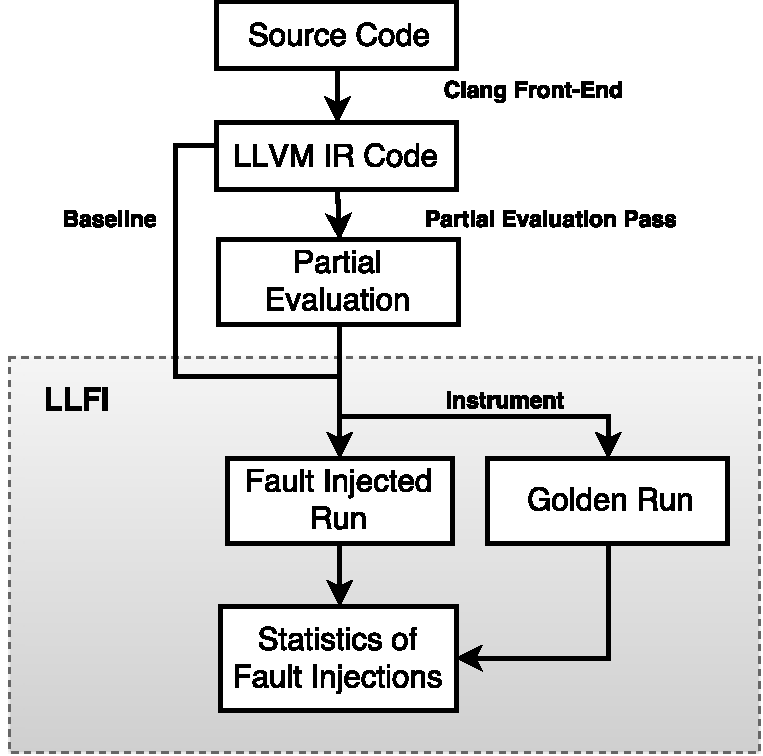
\includegraphics[keepaspectratio=true,width=0.8\columnwidth]{Evaluation_System}
  \caption{System Block Diagram of Evaluation Experimental Setup}
  \label{fig:evaluation_sys}
\end{figure}


We utilize the LLVM based fault injector, LLFI~\cite{LLFI} to carry out the experimentation.
LLFI injects software implemented faults into the program IR by modifying instruction or register values of the program at runtime.
It offers a range of simulated hardware and software faults that model real-world conditions~\cite{V2005}.
In this study, we select the following faults: bit flips, stuck-at-0, return value corruption, function call corruption, and invalid pointer.
Bit flips represent transient hardware faults, while stuck-at-0 represents permanent hardware faults. 
The rest of the faults represent transient software faults that occur as a result of a data corruption.
We omit permanent software faults in this study as discussed in Section~\ref{sec:fault_model}.

The injected faults are uniformly distributed throughout the program code.
Table~\ref{tab:faulttypes} describes how LLFI injects each fault.
We consider only activated faults, or those in which the modified data is read by the program, when measuring the fault outcome rate.


\begin{table}[htbp]
\small{
\begin{center}
    \begin{tabular}{|p{3cm}|p{5cm}|}
    \hline
    \textbf{Fault Type} & \textbf{LLFI Implementation} \\ \hline
    Bit Flip & Randomly flips a single bit in an arbitrary data value computed in the program  \\ \hline
    Stuck at 0 & Randomly sets a single bit to 0 in an arbitrary data value computed in the program  \\ \hline
    Return Value Corruption & Randomly corrupts the return value of a function call \\ \hline
    Function Call Corruption & Randomly corrupts the source register (i.e., parameter) of a function call \\ \hline
    Invalid Pointer & Randomly corrupts the returned pointer from malloc and calloc\\ \hline
    \hline
    \end{tabular}
    \end{center}
    }
    \caption{Description of faults injected using LLFI}
    \label{tab:faulttypes}
\end{table}
 

After running the experiment, we group and classify the results of the faulty program trials according to their failure outcome modes.
We determine whether the observations hold across failure modes and fault types. 
We make the following hypothesis with respect to the failure outcome rates.

\begin{hyp}
  \label{hyp:hypothesis}
The mean fault outcome rate ($f_p)$ of a program's partial evaluation is statistically equal to the mean fault outcome rate of the original program $(f_0$).
\end{hyp}

To realize this, we perform a two-sample t-test to determine whether the means are statistically equivalent to each other, within a 95\% confidence interval ($\delta_0$).
Our hypothesis expressed in formal terms is $H_1: f_0 - f_p < \delta_0 $.

In addition to measuring error resilience, we also measure the number of IR instructions in the partial evaluation and the original program respectively.
This allows us to compute the degree of specialization, $\psi$, defined as
\begin{align*}
\psi = \frac{P - P'}{P}
\end{align*}

where $P$ and $P'$ are the number of IR instructions in the original program, and its partial evaluation respectively.
The degree of specialization provides an approximate measure of the extent of code optimization and allows us to reason about correlations between partial evaluations and error resilience.


\subsection{Results}
\label{sec:results}
Forthcoming.
